\chapter{Vendor-neutral reference architecture}

\section{Engineering principles}

The proposed architecture uses ports and adapters. The application core owns task intake, routing, state transitions and evaluation policy. Provider adapters invoke existing coding agents; a workspace port allocates execution space; a verifier port evaluates candidate artifacts. Identity, approvals, storage and event export are infrastructure adapters. This avoids coupling business rules to a particular CLI or duplicating a native agent loop.\src{O6,A1,M1,G3}

\section{Implementation approach}

Define the runtime sequence: validate contract, allocate isolated workspace, select provider, execute within budget, inspect diff, run trusted verification, collect evidence, obtain external approval, hand off candidate to protected source control. Store task state in a durable service for production. Deploy workers without production credentials and place the verifier in a separately controlled runner. Use immutable artifact identifiers and authenticated service calls.

\section{Verification and limitations}

Quality attributes include bounded execution, auditability, isolation, portability and maintainability. Alternatives include a single native agent with CI for simple work, or a distributed coordinator for high concurrency. The example is a local teaching prototype, not a hardened production implementation.

Figure~\ref{fig:d23} illustrates the conceptual flow from the task sponsor through the isolated worker, verifier and approval gate. The edges describe the proposed integration or control relationship, not undocumented internal calls.

\begin{figure}[htbp]\centering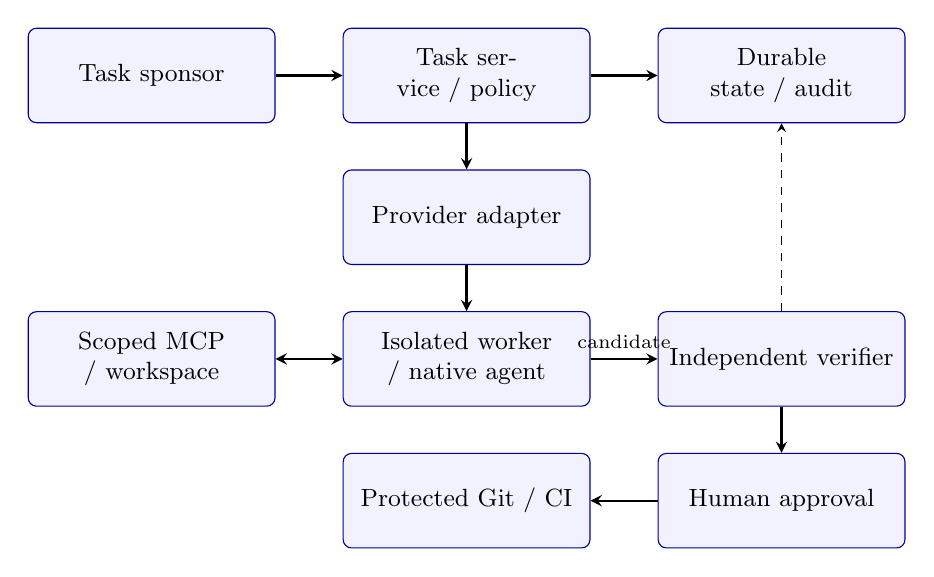
\begin{tikzpicture}[nodebox/.style={draw=blue!60!black,fill=blue!5,rounded corners=3pt,text width=29mm,minimum height=12mm,align=center,font=\small},>=stealth]
\node[nodebox] (sponsor) at (0,0) {Task sponsor};
\node[nodebox] (task) at (4,0) {Task service / policy};
\node[nodebox] (state) at (8,0) {Durable state / audit};
\node[nodebox] (adapter) at (4,-1.8) {Provider adapter};
\node[nodebox] (worker) at (4,-3.6) {Isolated worker / native agent};
\node[nodebox] (tools) at (0,-3.6) {Scoped MCP / workspace};
\node[nodebox] (verify) at (8,-3.6) {Independent verifier};
\node[nodebox] (review) at (8,-5.4) {Human approval};
\node[nodebox] (git) at (4,-5.4) {Protected Git / CI};
\draw[->,thick] (sponsor) -- (task);
\draw[->,thick] (task) -- (state);
\draw[->,thick] (task) -- (adapter);
\draw[->,thick] (adapter) -- (worker);
\draw[<->,thick] (worker) -- (tools);
\draw[->,thick] (worker) -- node[above,font=\scriptsize]{candidate} (verify);
\draw[->,thick] (verify) -- (review);
\draw[->,thick] (review) -- (git);
\draw[->,dashed] (verify) -- (state);
\end{tikzpicture}
\caption{Enterprise reference architecture (conceptual view).}\label{fig:d23}\end{figure}

\section{Viewpoints and operational contracts}
The context view identifies the sponsor, platform and source-control service. The functional view separates intake, routing, execution, verification and approval. The module view defines the provider, workspace, verifier and evidence ports. Runtime connectors carry a validated task, candidate and check report. The deployment view allocates the worker and verifier to independently controlled processes or hosts; the worker cannot administer either the verifier or the protected branch. The security view places authorization before external effects and requires task-scoped credentials. The information view associates evidence with task ID, baseline SHA, candidate digest and policy version. The operational view assigns recovery to the controller and incident escalation to the security owner.

The state machine begins at accepted, transitions to executing, and then to verification. A scoped and verified candidate enters awaiting-human-review. Only an external authenticated decision can move that candidate toward handoff. Scope denial and execution failure terminate immediately; verification failure permits a bounded repair. Every terminal state retains evidence. In a distributed deployment, use optimistic version checks for state transitions and idempotency keys for external effects. No successful verification transition can authorize a deployment.

\section{Chapter conclusion}

Apply the stated verification criteria before expanding the scope of this workflow. Record deviations, evidence and unresolved risks in the task record.
